\documentclass[journal]{IEEEtran}
\usepackage{amsmath,amssymb}
\usepackage{newtxtext}
\usepackage{newtxmath}
\usepackage{algorithmic}
\usepackage{booktabs}
\usepackage{array}
\usepackage{multirow}
\usepackage[caption=false,font=normalsize,labelfont=sf,textfont=sf]{subfig}
\usepackage{textcomp}
\usepackage{stfloats}
\usepackage{url}
\usepackage{verbatim}
\usepackage{graphicx}
\usepackage{cite}
\hyphenation{op-tical net-works semi-conduc-tor IEEE-Xplore}

\newcommand{\sg}{\operatorname{sg}}

\begin{document}

\title{Large-Model Prior and Causal Consistency for Unseen-Condition Multimodal Defect Recognition in Additive Manufacturing}

\author{Junwei~Gu, Jiahui~Guo, and Yu~Wang%
\thanks{Author affiliations, funding information, and the corresponding author note will be added in the final submission version.}}

\markboth{IEEE Transactions on Industrial Informatics,~Vol.~XX, No.~XX, Month~2026}%
{Gu \MakeLowercase{\textit{et al.}}: Large-Model Prior and Causal Consistency for Unseen-Condition Multimodal Defect Recognition in Additive Manufacturing}

\maketitle

\begin{abstract}
In-situ monitoring in metal additive manufacturing commonly yields multimodal observations, most notably visible and infrared signals. When training and test conditions differ, defect recognition models often rely on condition-dependent cues such as background texture or thermal-field distribution, and their performance drops sharply on unseen conditions. This paper presents the Multimodal Causal-Stable Qwen Network (MCSQ-Net) to address that problem. MCSQ-Net uses the visual encoder of a pretrained large model as a shared backbone, learns a unified multimodal fusion space, and introduces a causal consistency constraint that pulls same-class samples from different conditions closer in that space. A lightweight classification head is then used for defect category recognition, so that task adaptation remains limited while the pretrained visual prior is largely preserved. Experiments under both source-domain condition-held-out cross-validation and external transfer show clear gains over Prompt-Qwen and classical multimodal baselines. On Task-1, MCSQ-Net reaches a Macro-F1 of 0.8547 and a Balanced Accuracy of 0.8556; on Task-3 external transfer, it attains a Macro-F1 of 0.6067. Ablation results further show that causal consistency improves cross-condition representation quality, whereas aggressive unfreezing of the visual backbone weakens generalization. These findings suggest that, for small-sample industrial multimodal defect recognition, preserving large-model visual priors while explicitly enforcing cross-condition stability is an effective way to improve robustness under unseen conditions.
\end{abstract}

\begin{IEEEkeywords}
Selective laser melting, defect recognition, multimodal fusion, unseen-condition generalization, external transfer, large-model prior, causal consistency constraint.
\end{IEEEkeywords}

\section{Introduction}
\IEEEPARstart{M}{etal} additive manufacturing constructs complex parts layer by layer through the melting of metal powders and has been widely adopted in aerospace, medical devices, and tooling. Selective laser melting (SLM), as a representative process, involves complex physical phenomena such as melt-pool dynamics, heat transfer, and solidification \cite{ref_defect_formation_slm}. Variations in process parameters can directly lead to defects including pores, cracks, and geometric distortion \cite{ref_in_situ_monitoring_review}. Even minor process deviations may substantially affect the mechanical performance and service reliability of the final part.

Industrial systems commonly deploy visible-light cameras and infrared imagers to monitor metal additive manufacturing processes in a synchronized manner \cite{ref_lpbf_sensing_review,ref_intelligent_defect_pbf}. Visible imaging captures melt-pool morphology and surface texture, whereas infrared imaging reflects heat-input distribution and thermal-field evolution. Such multimodal observations provide complementary defect evidence. Existing monitoring methods, however, generally assume that training and test data follow the same distribution. When process parameters, equipment models, or powder batches change, recognition performance often degrades significantly.

This failure mode is closely tied to the tendency of deep models to exploit spurious correlations. Rather than learning defect-relevant structure, the model may latch onto superficial cues such as background texture, illumination pattern, or sensor noise. In multimodal monitoring for metal additive manufacturing, condition-specific thermal backgrounds can then be mistaken for defect evidence. The result is brittle performance once the operating condition changes. Learning recognition rules that remain valid from seen training conditions to unseen test conditions is therefore central to defect recognition in SLM.

Pretrained large visual models offer one plausible route forward. Because they are trained on large-scale visual and multimodal corpora, they provide strong priors for handling heterogeneous inputs and may help extract features that are less tied to a particular condition. Yet simple prompt-based adaptation is not enough in the present setting. Large-model priors do not automatically become reliable industrial defect evidence. What matters is how those priors are adapted so that cross-condition stability is preserved while complementary information from multiple sensors is still brought together effectively.

This paper proposes the Multimodal Causal-Stable Qwen Network (MCSQ-Net) for unseen-condition defect recognition in metal additive manufacturing. The model uses a pretrained large visual model as a shared cross-condition feature extractor, explicitly fuses visible and infrared observations, and regularizes the fused representation with a causal consistency constraint. The design follows a lightweight discriminative adaptation strategy, so that defect representations can be adapted to the task without overwriting the pretrained prior. The underlying assumption is straightforward: texture, brightness, and thermal background vary with process settings, whereas the essential characteristics of a defect should remain comparatively stable. By forcing same-class samples from different conditions to stay close in the fusion space, MCSQ-Net reduces its dependence on unstable environmental cues and learns a more reliable mapping from seen to unseen conditions.

The main contributions are threefold.
\begin{enumerate}
\item We verify the necessity of multimodal fusion for unseen-condition defect recognition. By comparing single-modality and multimodal configurations under cross-condition evaluation, we show that combining visible and infrared information improves adaptation to unseen devices and unseen process settings, thereby providing empirical guidance for sensor configuration in industrial monitoring systems.
\item We develop a large-model-prior-guided framework for unseen-condition defect recognition. The framework freezes the pretrained visual backbone and introduces a learnable multimodal fusion head for lightweight discriminative adaptation, balancing deployment efficiency and recognition accuracy. Experiments show that this strategy maintains stable detection performance in cross-device transfer scenarios.
\item We introduce a causal-stable representation learning mechanism. By enforcing consistency across same-class samples from different conditions, the model is encouraged to suppress background texture, thermal noise, and other environment-dependent cues, and to focus instead on the intrinsic characteristics of the defect itself. This mechanism improves generalization from seen to unseen conditions and provides a practical route toward robust industrial vision monitoring.
\end{enumerate}

\section{Related Work}
\subsection{Multimodal Defect Monitoring in Metal Additive Manufacturing}

In-situ monitoring for metal additive manufacturing has developed primarily along three lines: visible-light imaging, infrared thermography, and multi-sensor fusion \cite{ref_defect_formation_slm,ref_in_situ_monitoring_review,ref_lpbf_sensing_review,ref_intelligent_defect_pbf}. Across these lines, a consistent conclusion has emerged: multimodal observations describe defect formation from complementary perspectives, including morphology, thermal input, and process dynamics, and are therefore more informative than any single sensing modality.

Representative studies illustrate this trend. Wu \emph{et al.} \cite{ref_wu2024_multisensor} showed that multi-sensor monitoring improves quality-level recognition. Liu \emph{et al.} \cite{ref_liu2024_acoustic} inferred melt-pool visual characteristics from acoustic and thermal-radiation signals, offering a lower-cost alternative to direct high-speed imaging. Shen \emph{et al.} \cite{ref_shen2024_multisource} combined infrared images, top-view images, process parameters, and physical simulation results, while Li \emph{et al.} \cite{ref_li2024_transfer} examined the transferability of multimodal features across materials. Taken together, these studies establish the value of multimodal fusion for defect monitoring. Most of them, however, still assume that training and test samples are drawn from closely related distributions. Much less is known about the joint distribution shift introduced by changes in equipment, process parameters, and operating environments. The present work addresses that setting directly by seeking multimodal defect representations that remain stable under condition-disjoint evaluation.

\subsection{Large-Model Adaptation and Cross-Domain Generalization}

Pretrained large models provide a new source of prior knowledge for industrial anomaly and defect recognition. Recent work such as AnomalyGPT \cite{ref_anomalygpt}, Myriad \cite{ref_myriad}, OmniAD \cite{ref_omniad}, and AD-Copilot \cite{ref_ad_copilot} has demonstrated the potential of large models in industrial vision through prompt learning, expert-model integration, supervised fine-tuning, and visual context comparison. At the same time, lightweight adaptation strategies such as QLoRA and active learning \cite{ref_qlora_excavator,ref_vlm_active_learning} indicate that task specialization can be achieved in resource-constrained settings without full-parameter fine-tuning.

However, most existing methods focus on anomaly detection, localization, or few-shot adaptation within a single dataset. They seldom examine the cross-domain generalization problem created jointly by modality heterogeneity and condition shift in metal additive manufacturing. Once training and test conditions are strictly disjoint, prompting or conventional fine-tuning alone is often insufficient to ensure that the model learns genuinely stable defect evidence. In contrast, this paper uses the visual prior of a pretrained large model for unified multimodal encoding and introduces a cross-condition causal consistency constraint in the fusion space to improve recognition stability under unseen conditions.

\begin{figure*}[!t]
\centering
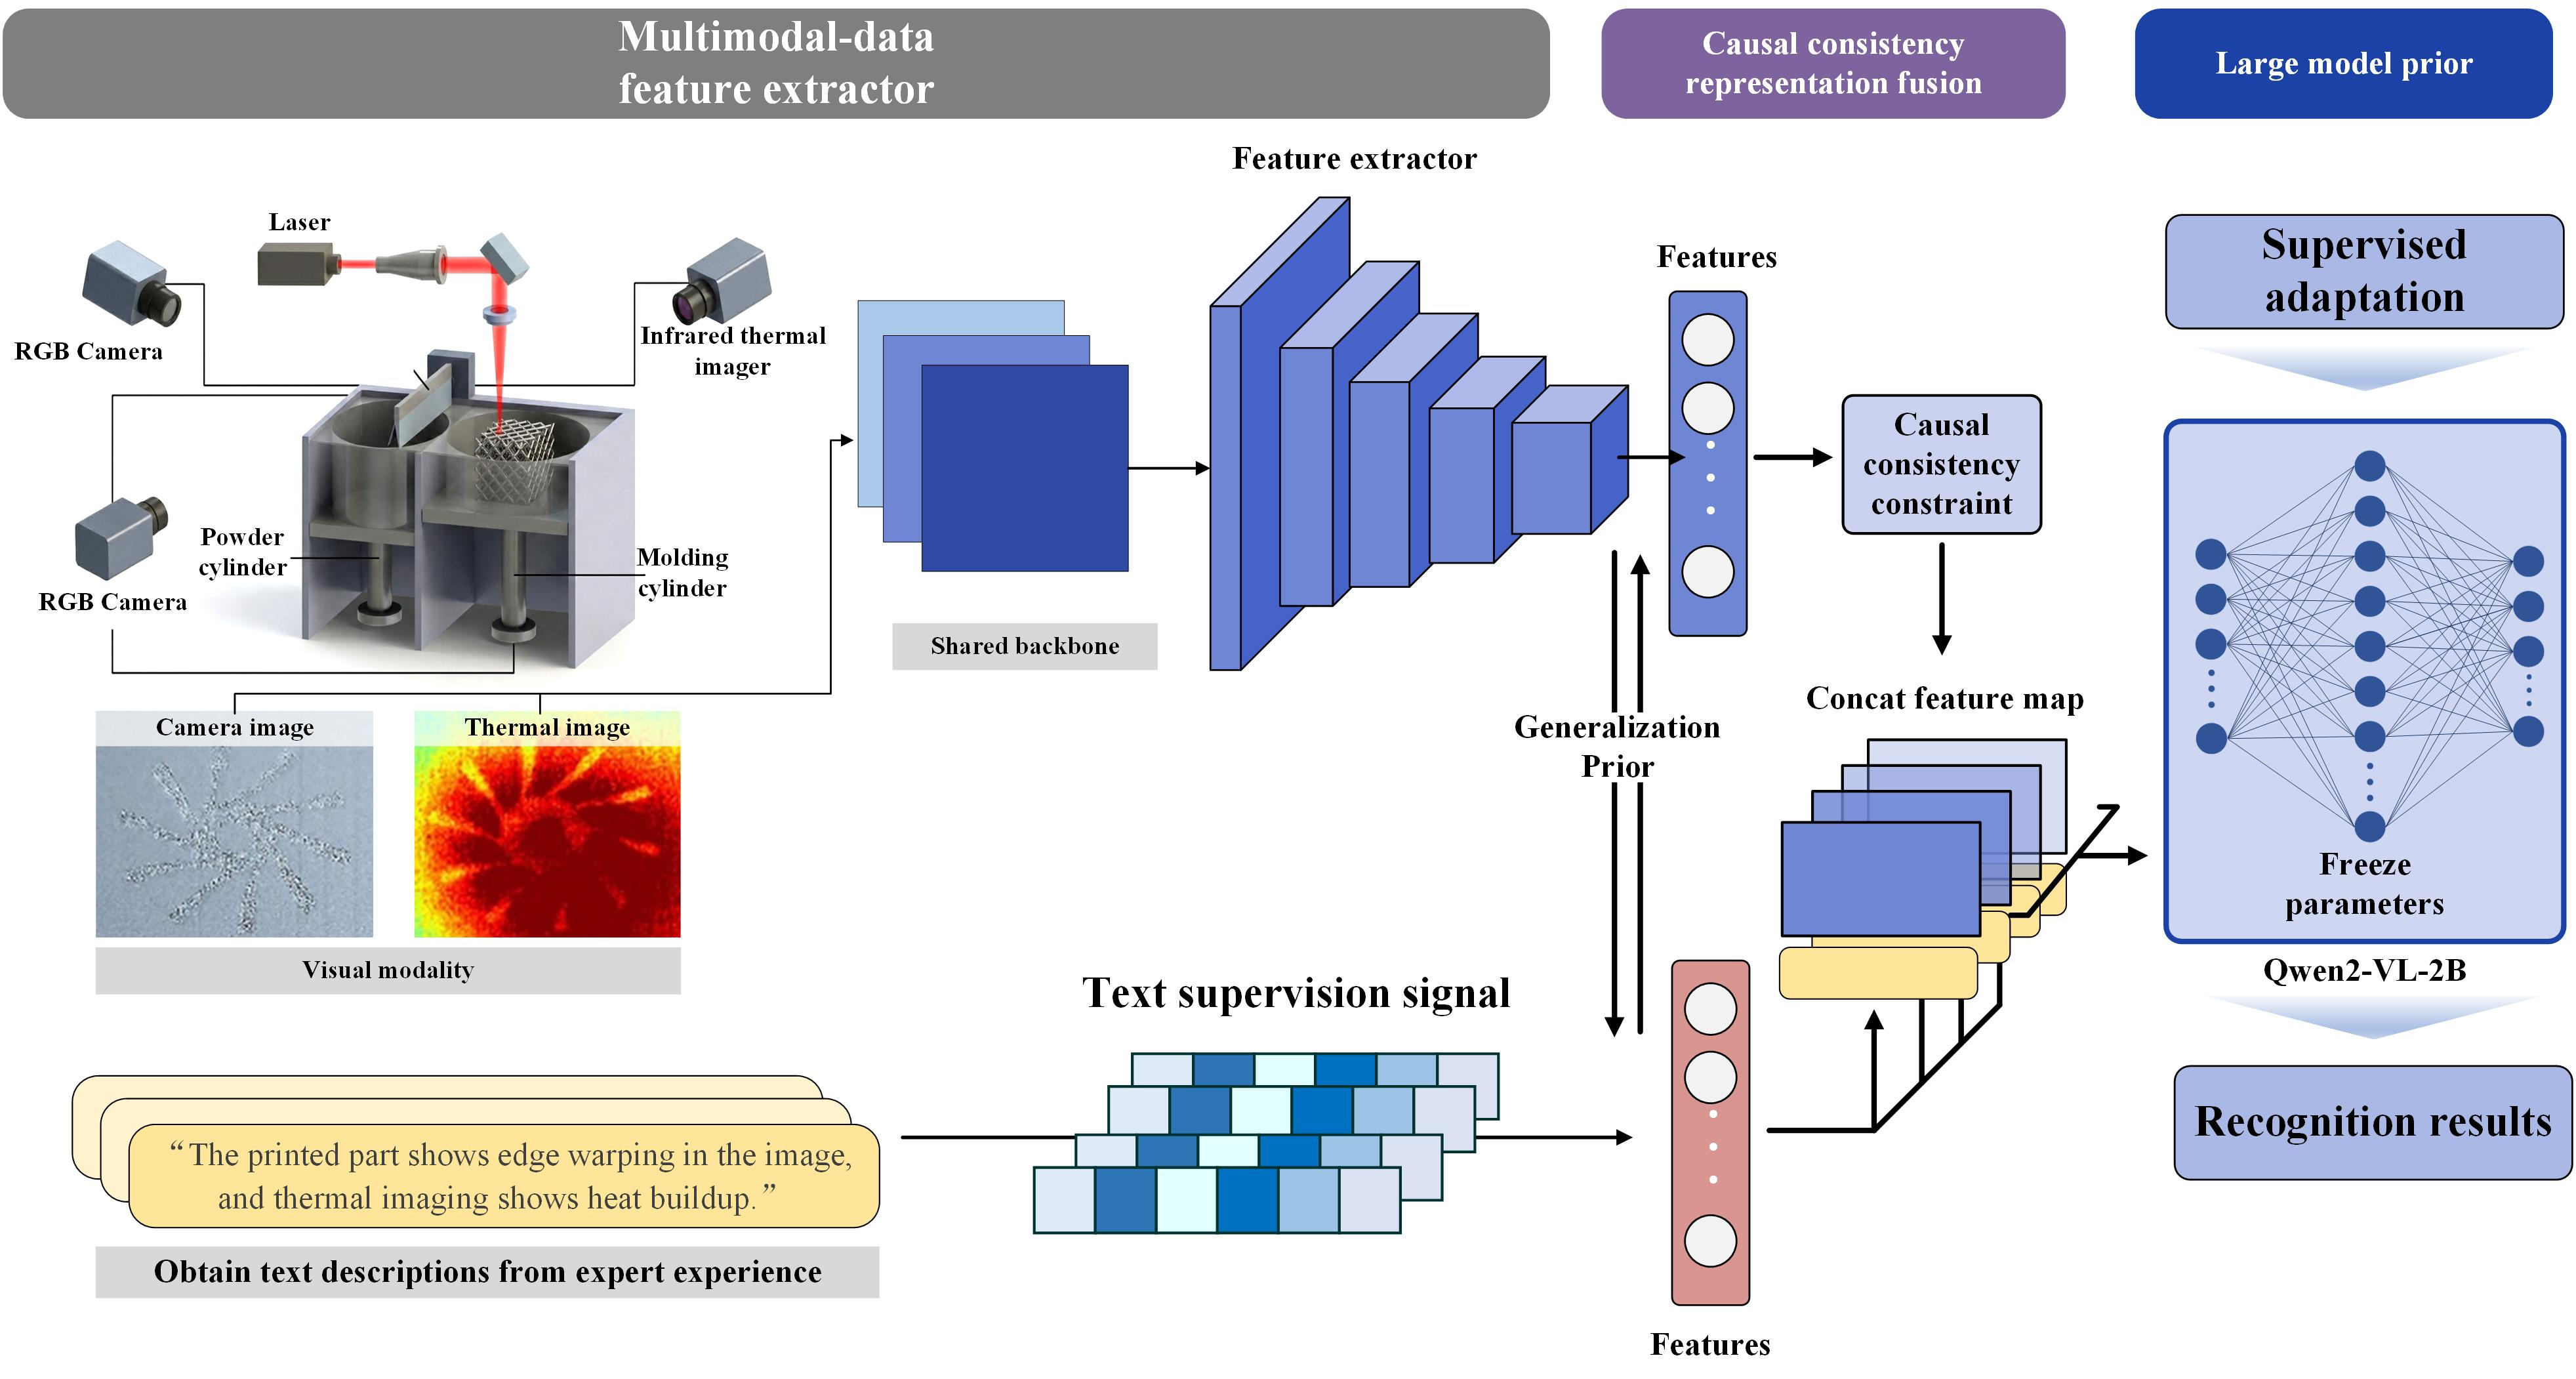
\includegraphics[width=0.95\textwidth]{fig1.jpg}
\caption{Overview of MCSQ-Net. The pipeline consists of shared visual encoding, multimodal causal-consistent fusion, and lightweight adaptation guided by large-model generalization priors.}
\label{fig:framework}
\end{figure*}

\section{Unseen-Condition Task Formulation}

Unseen-condition multimodal defect recognition in metal additive manufacturing can be formulated as a supervised classification problem under conditional extrapolation. For sample $i$, let the joint observation be $\mathbf{x}_i=\{\mathbf{x}_i^{(k)}\mid k\in\mathcal{M}_i\}\in\mathcal{X}$, where $\mathcal{M}_i$ denotes the set of available modalities. For visual and infrared observations, $\mathbf{x}_i^{(k)}\in\mathbb{R}^{H\times W\times C}$ denotes the input from the $k$th sensor, $y_i\in\mathcal{Y}$ is the defect label, $c_i\in\mathcal{C}$ is the condition identifier, and $\mathcal{X}$ is the multimodal observation space. The condition variable $c_i$ is used to represent external factors that change the observation distribution, including equipment configuration, process parameters, printing task, and material state. Unlike conventional in-distribution classification, the training set $\mathcal{D}_{\mathrm{train}}=\{(\mathbf{x}_i,y_i,c_i)\}_{i=1}^{N}$ and the test set $\mathcal{D}_{\mathrm{test}}$ come from condition sets $\mathcal{C}_{\mathrm{train}}$ and $\mathcal{C}_{\mathrm{test}}$, respectively, with $\mathcal{C}_{\mathrm{train}}\cap\mathcal{C}_{\mathrm{test}}=\varnothing$. The model therefore faces not only new instances at test time, but also systematic distribution shifts caused by changes in equipment, process settings, and task conditions.

Under this setting, the model must learn a classifier $f:\mathcal{X}\rightarrow\mathcal{Y}$ solely from $\mathcal{D}_{\mathrm{train}}$ while maintaining low risk on unseen conditions:
\begin{equation}
\mathcal{R}_{\mathrm{uc}}(f)=\mathbb{E}_{(\mathbf{x},y,c)\sim P_{\mathrm{test}}}\left[\ell\!\left(f(\mathbf{x}),y\right)\right], \quad c\in\mathcal{C}_{\mathrm{test}},
\label{eq:uc_risk}
\end{equation}
where $\ell(\cdot,\cdot)$ is the classification loss, $\mathcal{R}_{\mathrm{uc}}$ denotes the unseen-condition risk, and $P_{\mathrm{test}}$ is the test-time data distribution. This objective is difficult because multimodal observations simultaneously contain stable discriminative factors related to defect formation and unstable background statistics or sensor-response differences induced by condition changes. Direct empirical risk minimization can exploit the latter to fit the training set, thereby encoding condition-dependent superficial correlations into the decision rule and causing failure on $\mathcal{C}_{\mathrm{test}}$. Based on this task definition, the proposed method addresses three aspects: unified representation of heterogeneous observations, extraction of condition-stable features, and transfer of large-model priors.

\section{Proposed Method}

To address the difficulties of heterogeneous multimodal representation, condition-dependent decision drift, and limited extrapolation under scarce labeled data, this paper proposes MCSQ-Net. For sample $i$, let its effective modality set be $\mathcal{M}_i=\{m_1,\dots,m_{K_i}\}$, where $K_i$ is the number of modalities involved in fusion. Rather than using a pretrained large model directly for prompt-based closed-set classification, MCSQ-Net takes its visual encoding component as a shared feature extractor and successively performs multimodal representation learning, cross-condition consistent fusion, and lightweight discriminative adaptation. In this way, the method seeks to suppress condition-induced representation drift while preserving as much of the pretrained prior as possible. The overall framework is shown in Fig.~\ref{fig:framework}.

\subsection{Multimodal Feature Extraction}

Different sensors exhibit different imaging mechanisms and statistical properties. Training a separate encoder for each modality can easily cause the model to memorize condition-related textures under limited supervision rather than stable defect cues. To mitigate this issue, MCSQ-Net shares a single pretrained large-model visual backbone $f_{\theta_v}$ across all modalities, first mapping heterogeneous observations into a unified semantic space and then constructing modality-level representations within that space.

For any modality $m\in\mathcal{M}_i$, let the input observation be $\mathbf{x}_i^{(m)}$. The shared visual encoder produces the spatial feature sequence
\begin{equation}
\mathbf{E}_i^{(m)} = f_{\theta_v}\!\left(\mathbf{x}_i^{(m)}\right)
= \left[\mathbf{e}_{i,1}^{(m)},\dots,\mathbf{e}_{i,P_i^{(m)}}^{(m)}\right]^\top
\in \mathbb{R}^{P_i^{(m)} \times d_v},
\label{eq:vision_features}
\end{equation}
where $d_v$ is the feature dimension, $P_i^{(m)}$ is the number of retained local features after spatial compression in the visual backbone, and $\mathbf{e}_{i,p}^{(m)}$ is the local visual feature at the $p$th spatial position. Since the downstream fusion module requires fixed-length inputs, the spatial feature sequence is mean-pooled to obtain a modality-level representation:
\begin{equation}
\mathbf{z}_i^{(m)} = \frac{1}{P_i^{(m)}} \sum_{p=1}^{P_i^{(m)}} \mathbf{e}_{i,p}^{(m)} \in \mathbb{R}^{d_v}.
\label{eq:modal_pooling}
\end{equation}
Here, $\mathbf{z}_i^{(m)}$ is the global semantic vector of modality $m$. This operation compresses a variable-length spatial sequence into a fixed-length vector and thereby reduces scale differences across modalities. For all input modalities of sample $i$, the modality-level feature group is
\begin{equation}
\mathbf{Z}_i = \left[\mathbf{z}_i^{(m_1)},\dots,\mathbf{z}_i^{(m_{K_i})}\right] \in \mathbb{R}^{K_i \times d_v}.
\label{eq:modal_stack}
\end{equation}
where $K_i$ is the number of modalities actually involved in fusion. In the main setting, the shared visual backbone remains frozen and is used only as a unified feature extractor. This choice preserves the pretrained visual prior and provides a more stable basis for the subsequent cross-condition consistency constraint.

\begin{figure}[!t]
\centering
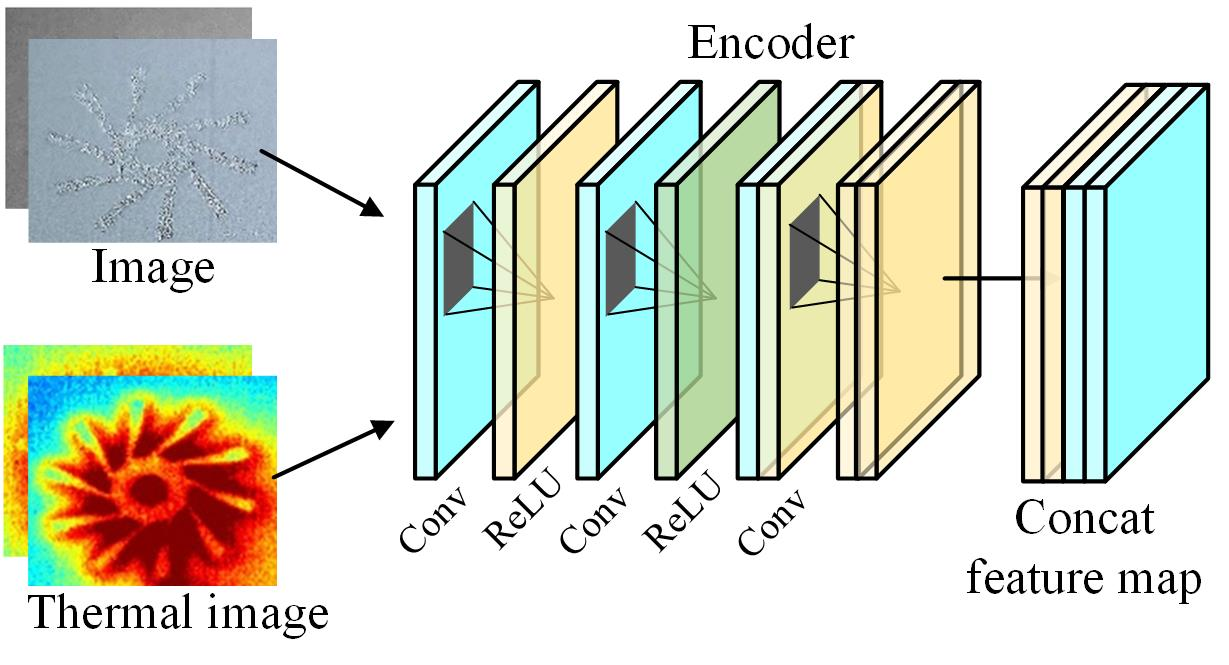
\includegraphics[width=0.4\textwidth]{fig2.jpg}
\caption{Multimodal feature extraction module.}
\label{fig:feature_extractor}
\end{figure}

\subsection{Causal-Consistent Representation Fusion}

After obtaining modality-level vectors, directly sending them into a classifier would still allow the model to encode brightness bias, thermal background, and texture noise as decision cues. The goal of this stage is therefore not to design an increasingly complex fusion network, but to explicitly constrain condition-stable factors at the fused representation level so that the representation is more tightly tied to the defect itself.

Specifically, the modality vectors of sample $i$ are first concatenated along the feature dimension to form the joint description
\begin{equation}
\mathbf{g}_i = \mathrm{Concat}\!\left(\mathbf{z}_i^{(m_1)}, \dots, \mathbf{z}_i^{(m_{K_i})}\right) \in \mathbb{R}^{K_i d_v}.
\label{eq:concat}
\end{equation}
The fused representation is then obtained by mapping this joint description into a common fusion space:
\begin{equation}
\mathbf{h}_i = \phi_{\theta_f}\!\left(\mathrm{LN}(\mathbf{g}_i)\right) \in \mathbb{R}^{d_h}.
\label{eq:fusion}
\end{equation}
where $\mathrm{LN}(\cdot)$ denotes LayerNorm and $d_h$ is the fusion-space dimension. The fusion head $\phi_{\theta_f}$ is only responsible for feature compression and cross-modal recombination; suppression of condition-dependent spurious correlations is mainly achieved by the subsequent consistency constraint.

The causal consistency constraint is built on the assumption that, for the same defect category, background texture, brightness distribution, and thermal response may vary across conditions, whereas defect morphology and abnormal thermal signatures that determine class identity should remain stable. To make this stable component comparable in the fusion space, the fused vector is first $\ell_2$-normalized:
\begin{equation}
\bar{\mathbf{h}}_i = \frac{\mathbf{h}_i}{\|\mathbf{h}_i\|_2} \in \mathcal{S}^{d_h-1}.
\label{eq:norm}
\end{equation}
The normalized vector $\bar{\mathbf{h}}_i$ retains only directional information. Consequently, its inner product with another normalized vector directly corresponds to cosine similarity, which is more suitable for measuring semantic consistency across conditions.

For each sample, a same-class but different-condition reference set is constructed. For sample $i$, define the cross-condition positive pool as
\begin{equation}
\Omega_i = \left\{ j \mid j \neq i,\; y_j = y_i,\; c_j \neq c_i \right\}.
\label{eq:pool}
\end{equation}
Here, $y_j = y_i$ ensures that the two samples belong to the same defect category, and $c_j \neq c_i$ ensures that they come from different conditions. The resulting consistency relation is therefore defined between sample-level cross-condition positive pairs rather than between different modalities. If a sample does not have an available positive pair, it does not contribute to the consistency loss in the current mini-batch.

For the subset of anchors in a mini-batch $\mathcal{B}$ that have valid positives, denoted by $\mathcal{B}^{+}=\{i\in\mathcal{B}\mid\Omega_i\neq\varnothing\}$, one positive $\pi(i)$ is sampled from $\Omega_i$. The causal consistency loss is then written as
\begin{equation}
\mathcal{L}_{\mathrm{cc}} =
\frac{1}{|\mathcal{B}^{+}|}
\sum_{i\in\mathcal{B}^{+}}
\left(
1-\bar{\mathbf{h}}_i^{\top}\sg\!\left(\bar{\mathbf{h}}_{\pi(i)}\right)
\right),
\label{eq:cc}
\end{equation}
where $\sg(\cdot)$ denotes the stop-gradient operator used to block gradient backpropagation through the reference branch. Since both $\bar{\mathbf{h}}_i$ and $\bar{\mathbf{h}}_{\pi(i)}$ are normalized, their inner product directly corresponds to cosine similarity. Thus, the role of \eqref{eq:cc} is to pull together fused representations of same-class samples from different conditions, keeping consistent defect semantics close while reducing the interference of condition differences on the decision boundary.

\begin{figure}[!t]
\centering
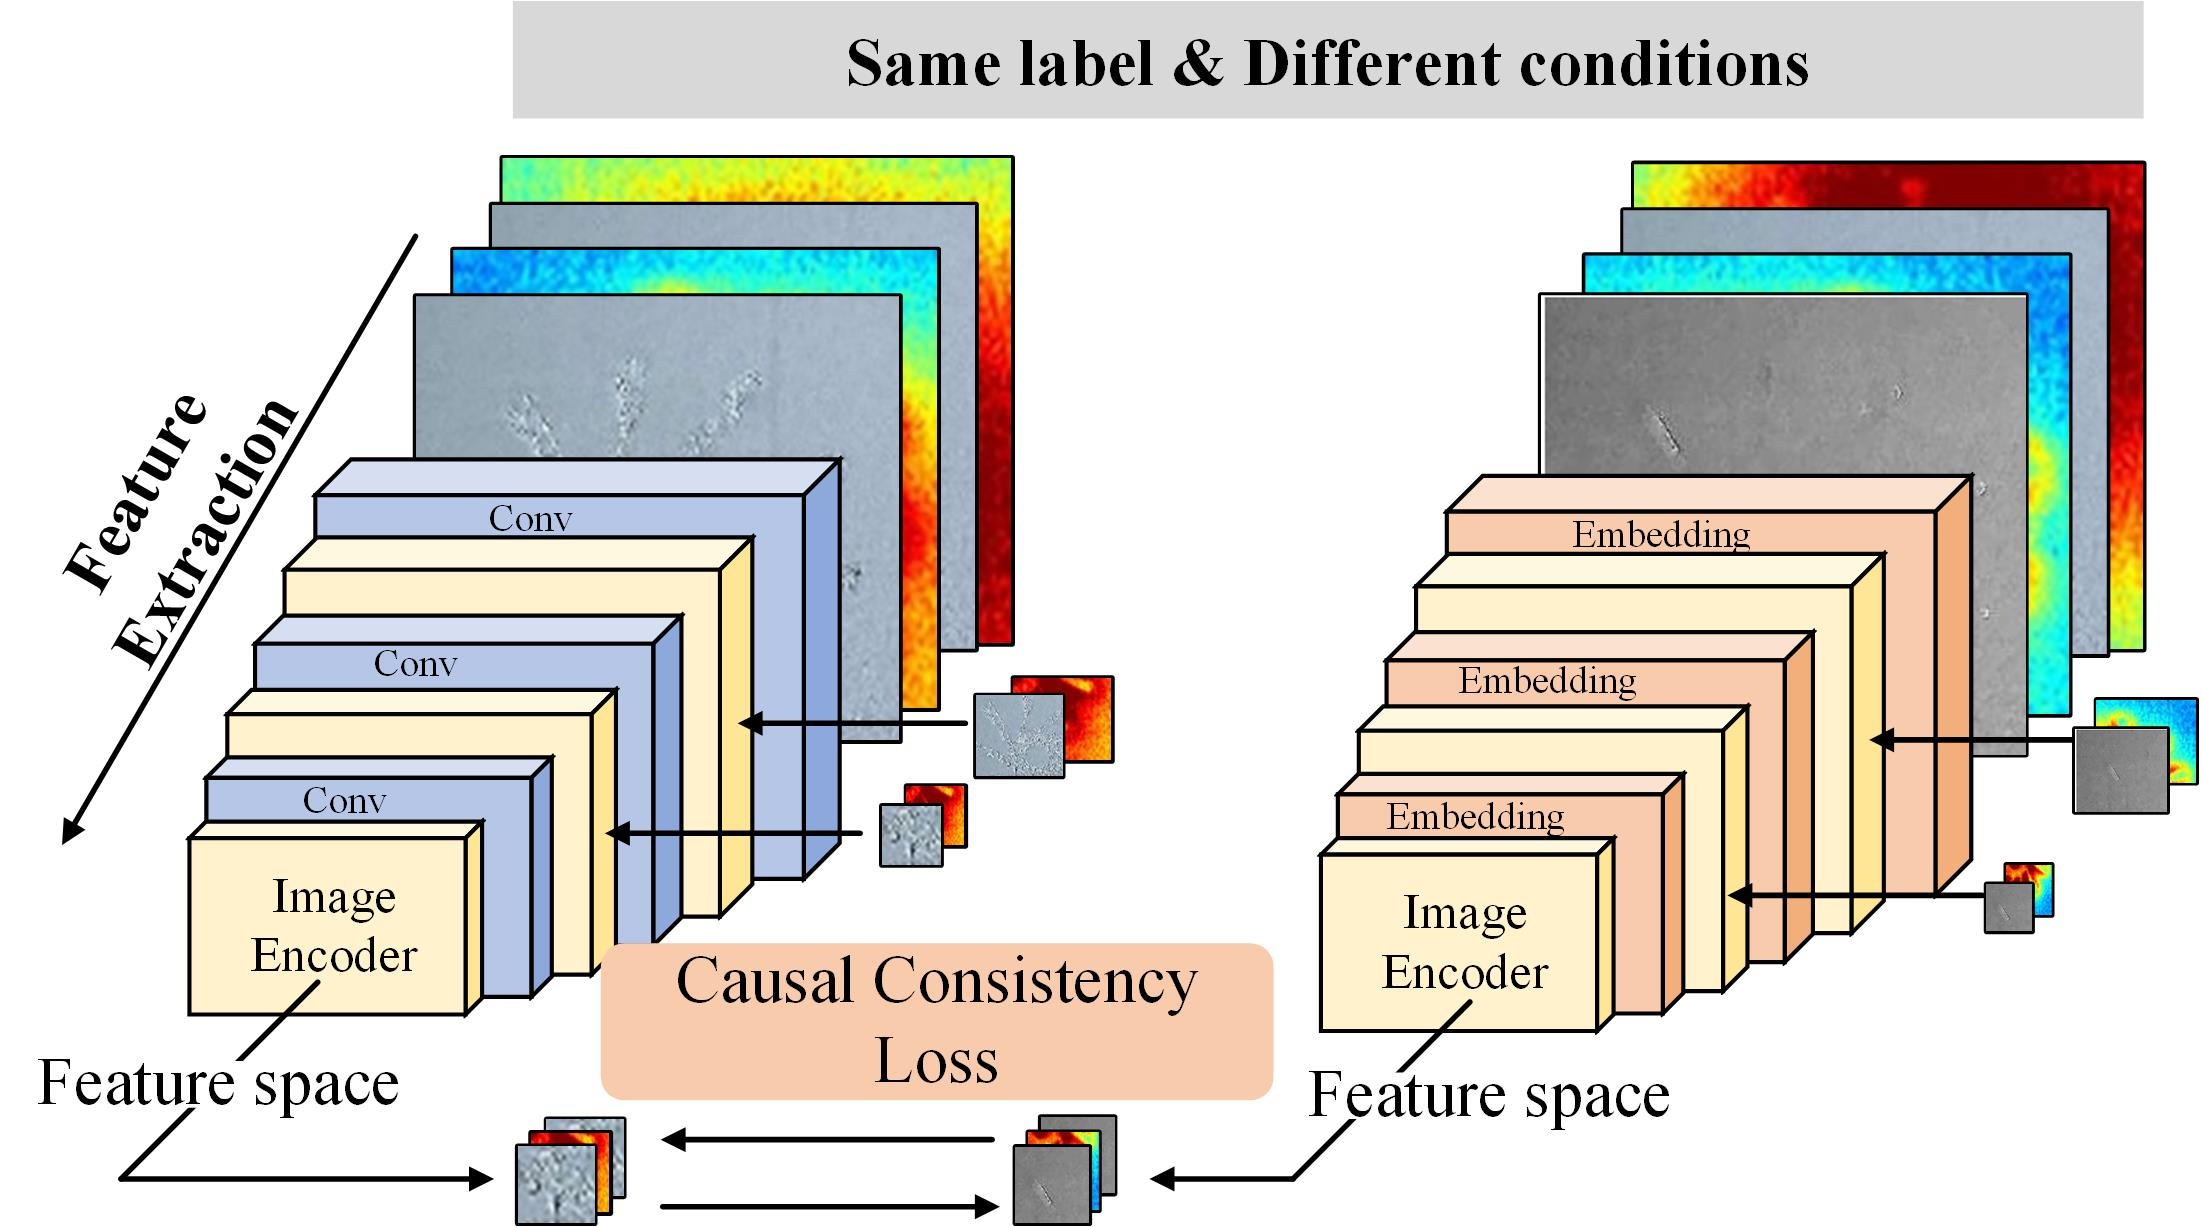
\includegraphics[width=0.45\textwidth]{fig3.jpg}
\caption{Causal-consistent fusion module.}
\label{fig:causal_fusion}
\end{figure}

\subsection{Lightweight Adaptation Guided by Large-Model Priors}

After obtaining the fused representation, the generalization prior formed by the pretrained large model on open-domain visual data still needs to be converted into category-specific defect discrimination. Direct end-to-end fine-tuning of the visual backbone would easily rewrite that prior into local experience tied to a small number of training conditions, whereas no task adaptation at all would make it difficult to form stable category boundaries. Therefore, under the proposed setting, the visual backbone remains frozen and only the fusion head and classification head are updated, yielding lightweight task adaptation with a small number of trainable parameters.

Concretely, the classification score vector is computed from the fused representation $\mathbf{h}_i$ as
\begin{equation}
\boldsymbol{\ell}_i = \mathbf{W}_c \mathbf{h}_i + \mathbf{b}_c \in \mathbb{R}^{|\mathcal{Y}|},
\label{eq:scores}
\end{equation}
where $\mathbf{W}_c \in \mathbb{R}^{|\mathcal{Y}| \times d_h}$ and $\mathbf{b}_c \in \mathbb{R}^{|\mathcal{Y}|}$ are the weight matrix and bias vector of the classifier, respectively, $|\mathcal{Y}|$ is the number of defect categories, and $\ell_{i,k}$ is the unnormalized score of sample $i$ for class $k$. The classification loss is standard cross-entropy:
\begin{equation}
\mathcal{L}_{\mathrm{cls}} =
-\frac{1}{|\mathcal{B}|}\sum_{i \in \mathcal{B}}
\log
\frac{\exp(\ell_{i,y_i})}{\sum_{k=1}^{|\mathcal{Y}|}\exp(\ell_{i,k})},
\label{eq:ce}
\end{equation}
where $|\mathcal{B}|$ denotes the batch size. $\mathcal{L}_{\mathrm{cls}}$ learns class-separating decision boundaries, whereas $\mathcal{L}_{\mathrm{cc}}$ suppresses condition-induced representation drift; the two objectives correspond to class separability and cross-condition stability, respectively.

In the parameter update strategy, the pretrained visual backbone is frozen, and only the fusion-head parameters $\theta_f$ and the classifier parameters $\theta_c=(\mathbf{W}_c,\mathbf{b}_c)$ are updated. This lightweight adaptation strategy confines task-specific updates to a small set of added modules and thus preserves the large-model prior as much as possible under limited supervision.

Combining the above components, the final optimization objective is
\begin{equation}
\mathcal{L} = \mathcal{L}_{\mathrm{cls}} + \lambda \mathcal{L}_{\mathrm{cc}},
\label{eq:total}
\end{equation}
where $\lambda$ is the weight of the consistency constraint. Equation~\eqref{eq:total} indicates that optimization does not only pursue class separability on the training set, but also requires the fused representation to remain stable under condition variation.

\subsection{Training Procedure and Overall Architecture}

Training follows standard mini-batch gradient descent. Each update consists of four steps: shared visual encoding, multimodal fusion, cross-condition consistency alignment, and discriminative optimization. The shared visual backbone first extracts modality-level vectors, the fusion head produces $\mathbf{h}_i$ and $\bar{\mathbf{h}}_i$, and then $\mathcal{L}_{\mathrm{cls}}$ and $\mathcal{L}_{\mathrm{cc}}$ are jointly computed to update the trainable parameters. Table~\ref{tab:method_train_algo} presents the training pseudocode, and Table~\ref{tab:method_model_arch} summarizes the key architectural configuration. Detailed training hyperparameters are deferred to the experimental settings.

\begin{table}[!t]
\centering
\caption{MCSQ-Net Training Procedure}
\label{tab:method_train_algo}
\footnotesize
\setlength{\tabcolsep}{0pt}
\begin{tabular*}{\columnwidth}{@{\extracolsep{\fill}}p{0.985\columnwidth}@{}}
\toprule
\textbf{Training Procedure} \\
\midrule
\begin{minipage}[t]{0.985\columnwidth}
\begin{algorithmic}[1]
\STATE \textbf{Input:} training set $\mathcal{D}_{\mathrm{train}}$, validation set $\mathcal{D}_{\mathrm{val}}$, shared visual backbone $f_{\theta_v}$, fusion head $\phi_{\theta_f}$, classifier $(\mathbf{W}_c,\mathbf{b}_c)$, and weight $\lambda$
\STATE \textbf{Initialization:} freeze all visual layers of $f_{\theta_v}$; build same-class cross-condition positive pools for training samples according to labels and \texttt{condition\_uid}
\FOR{epoch $=1$ to $E$}
    \FOR{mini-batch $\mathcal{B}$}
        \STATE Read the input observations of each sample according to the current modality configuration and pass them through the shared visual backbone
        \STATE Mean-pool the spatial feature sequence of each modality to obtain modality-level vectors $\mathbf{z}_i^{(m)}$
        \STATE Concatenate all modality vectors and pass them through the fusion head to obtain $\mathbf{h}_i$ and its normalized form $\bar{\mathbf{h}}_i$
        \STATE Compute classification scores with the classifier and obtain the classification loss $\mathcal{L}_{\mathrm{cls}}$
        \IF{valid positive pairs exist in the batch}
            \STATE Compute the consistency loss $\mathcal{L}_{\mathrm{cc}}$ according to the same-class cross-condition matching relation
        \ELSE
            \STATE Set $\mathcal{L}_{\mathrm{cc}} \leftarrow 0$
        \ENDIF
        \STATE Compute the total loss $\mathcal{L}=\mathcal{L}_{\mathrm{cls}}+\lambda \mathcal{L}_{\mathrm{cc}}$
        \STATE Backpropagate and update the trainable parameters
    \ENDFOR
    \STATE Evaluate the current model on the validation set and save the best checkpoint according to the main metric
    \IF{no improvement over several epochs}
        \STATE Trigger early stopping
    \ENDIF
\ENDFOR
\STATE \textbf{Output:} the best model parameters on the validation set and the corresponding test results
\end{algorithmic}
\end{minipage} \\
\bottomrule
\end{tabular*}
\end{table}

\begin{table*}[!t]
\centering
\caption{Key Architectural Configuration of MCSQ-Net}
\label{tab:method_model_arch}
\footnotesize
\setlength{\tabcolsep}{4pt}
\begin{tabular*}{\textwidth}{@{\extracolsep{\fill}}>{\raggedright\arraybackslash}p{0.17\textwidth}>{\raggedright\arraybackslash}p{0.47\textwidth}>{\raggedright\arraybackslash}p{0.28\textwidth}@{}}
\toprule
Module & Structure & Role \\
\midrule
Shared visual backbone & Pretrained visual encoder, $d_v=1536$, all visual layers frozen & Extract unified modality features \\
Modality aggregation & Mean pooling, $\mathbf{z}_i^{(m)}\in\mathbb{R}^{d_v}$ & Generate modality-level representations \\
Feature concatenation & $\mathbf{g}_i=\mathrm{Concat}(\mathbf{z}_i^{(m_1)},\dots,\mathbf{z}_i^{(m_{K_i})})\in\mathbb{R}^{K_i d_v}$ & Preserve complementary multimodal information \\
Fusion head & $\mathrm{LN}+\mathrm{Linear}(K_i d_v,512)+\mathrm{GELU}+\mathrm{Dropout}(0.1)+\mathrm{Linear}(512,512)+\mathrm{GELU}$ & Compress and reorganize fused features \\
Consistency constraint & Same-label cross-condition pairing, cosine consistency loss, $\lambda=0.1$ & Suppress condition-induced shift \\
Classifier & $\mathrm{Linear}(512,|\mathcal{Y}|)$ & Output defect-class scores \\
Lightweight adaptation & Freeze the visual backbone and train only $\{\theta_f,\theta_c\}$ & Preserve the large-model generalization prior \\
\bottomrule
\end{tabular*}
\end{table*}

\section{Experiments and Analysis}
\subsection{Experimental Settings}

The experimental data were collected from a self-built open SLM in-situ monitoring platform, as illustrated in Fig.~\ref{fig:platform_setup}. The platform consists of a 500~W single-mode continuous-wave fiber laser, a galvanometer scanning system, and PBAM programmable control software, allowing real-time adjustment of key process parameters such as laser power and scanning speed. The build process is conducted under high-purity argon protection, with oxygen concentration controlled below 0.1\%. To acquire multimodal process signals, the platform is equipped with two KM2010-3660 industrial cameras and one Optris PI 08M short-wave infrared imager, which record top-view and side-view visible images as well as vertical infrared thermal fields, respectively, with frame-level synchronization achieved through external TTL triggering. The resulting dataset contains visual modalities, the infrared modality, and corresponding condition information, and is used for unseen-condition defect recognition evaluation.

\begin{figure}[!t]
\centering
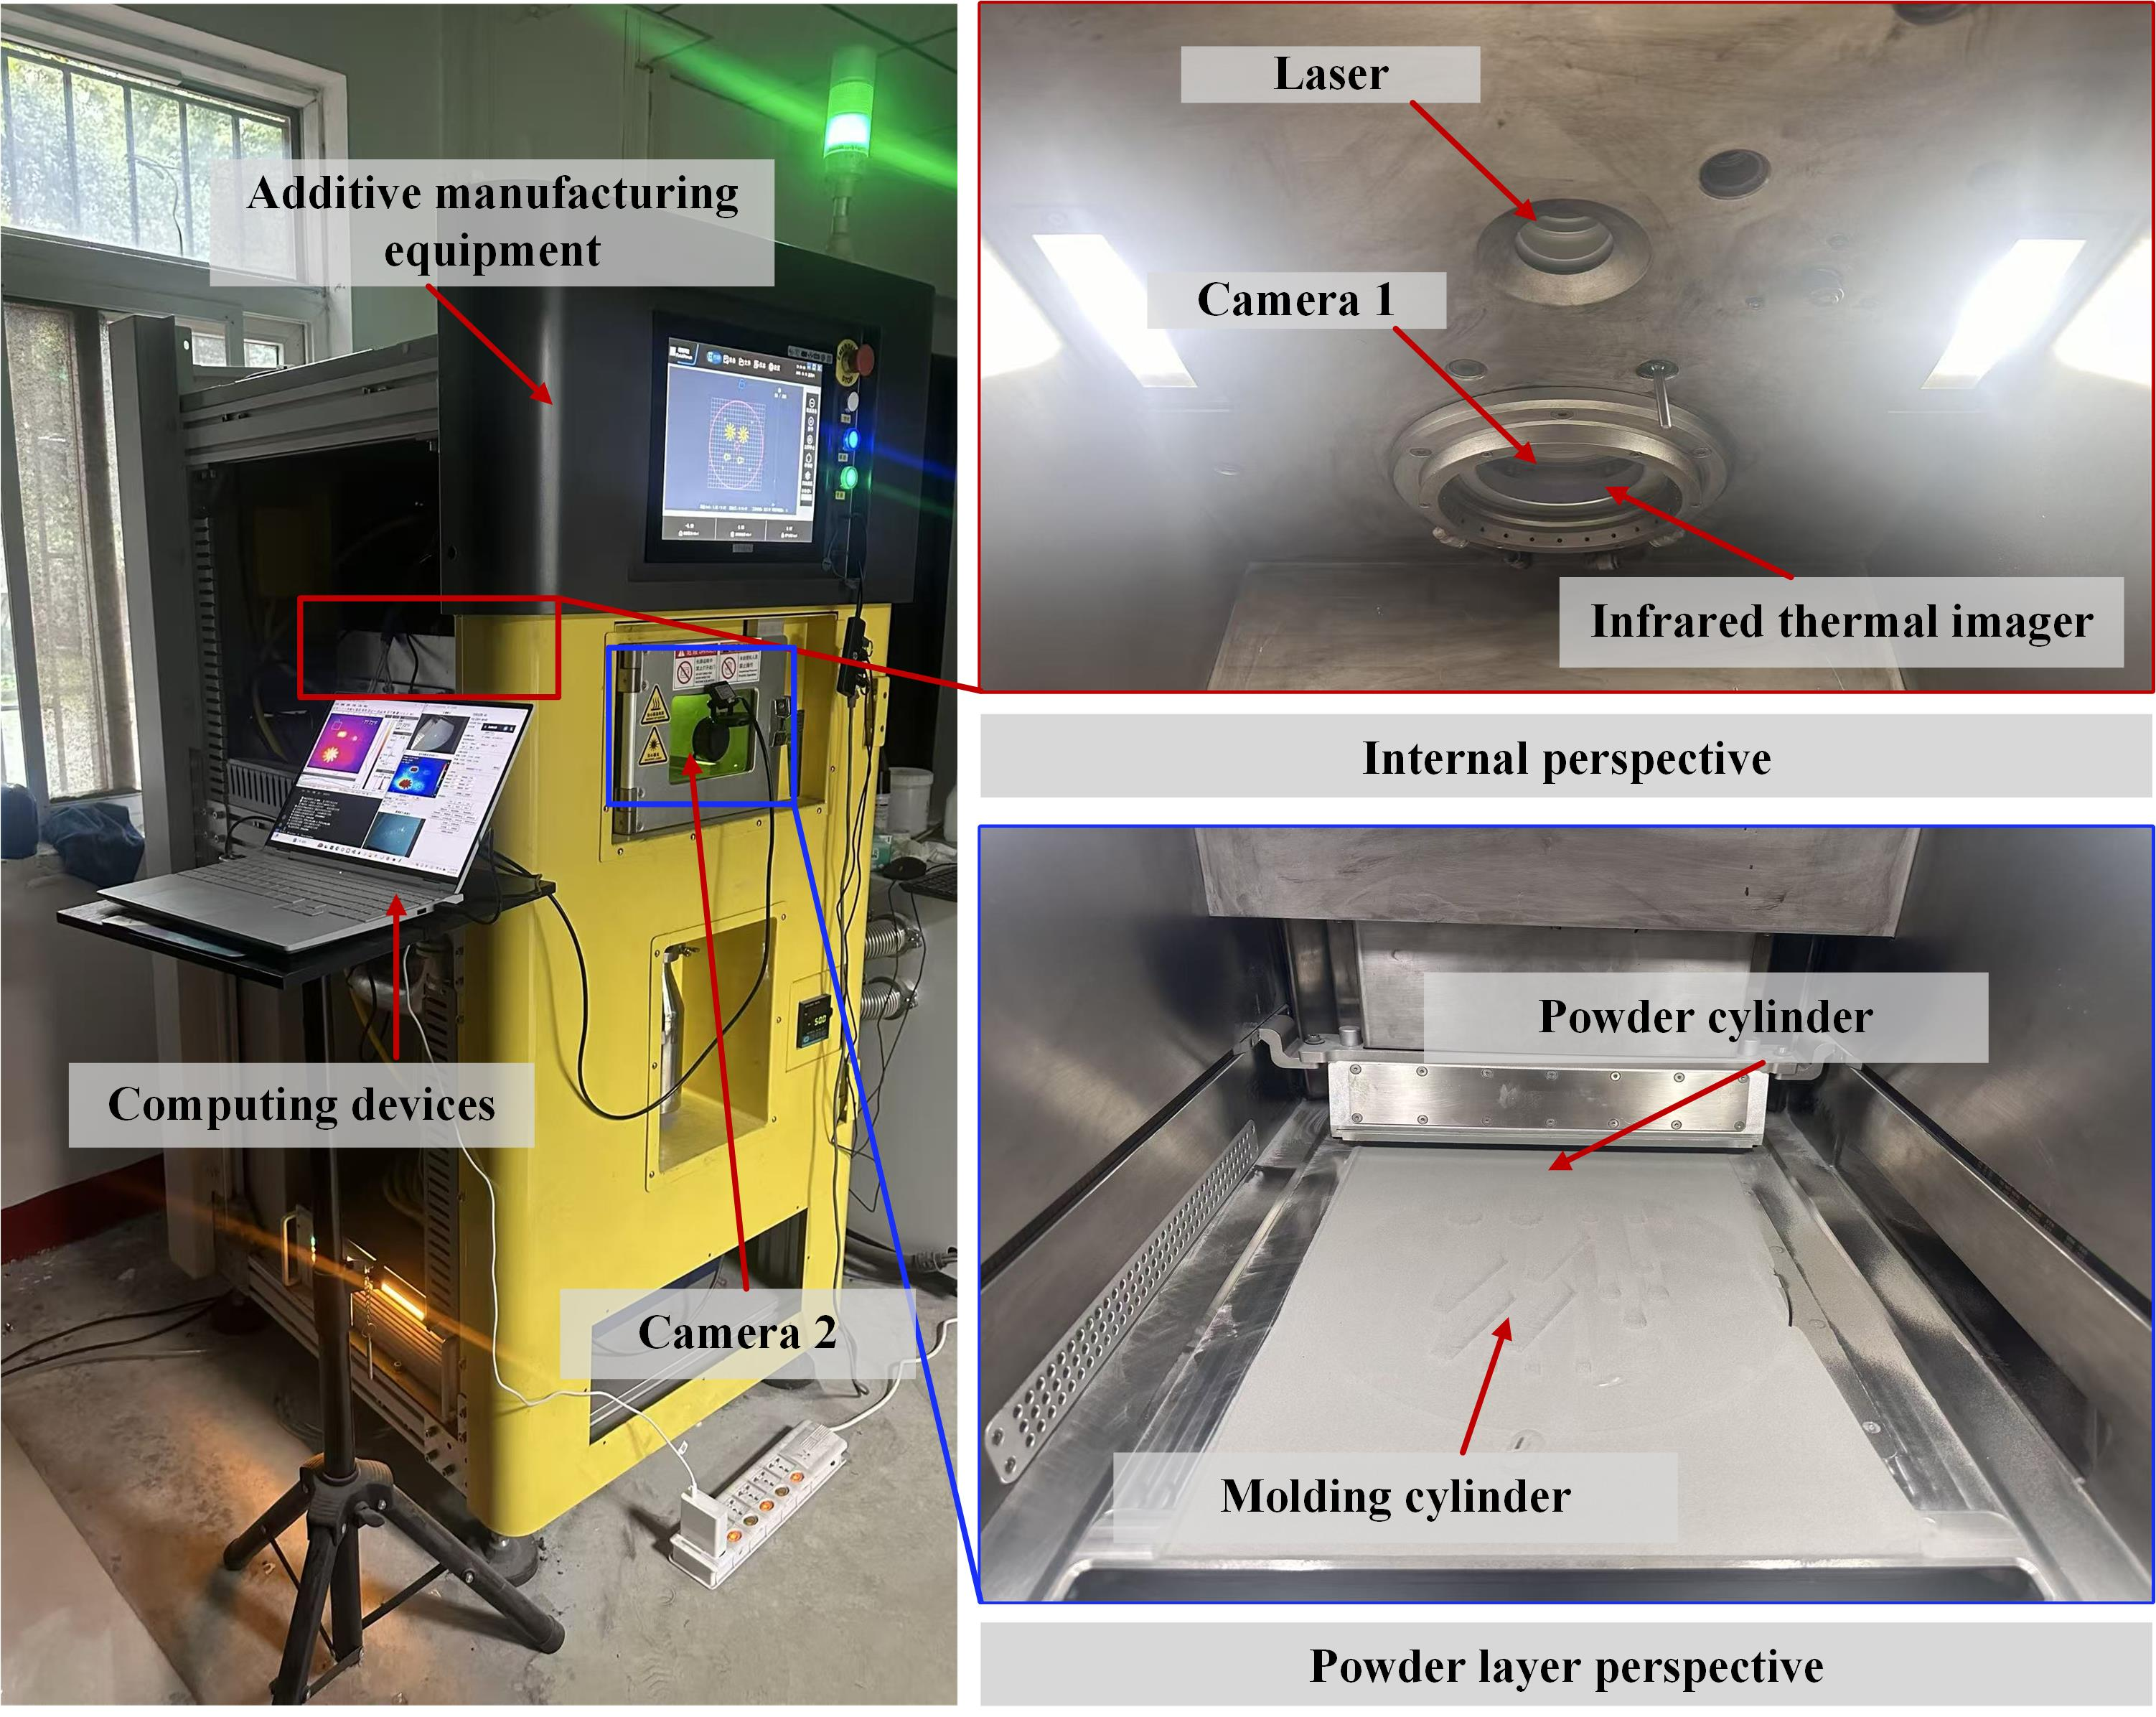
\includegraphics[width=0.45\textwidth]{fig4.jpg}
\caption{Open SLM in-situ monitoring platform and multi-sensor acquisition system. The final version will show the laser processing unit, the control system, and the dual-vision and infrared sensing array.}
\label{fig:platform_setup}
\end{figure}

The proposed method uses the visual backbone of Qwen2-VL-2B-Instruct. The fusion dimension is set to 512 and dropout to 0.1. Training uses AdamW with a learning rate of $3\times10^{-4}$, weight decay of $10^{-4}$, cosine scheduling, mixed-precision optimization, batch size 4, and early stopping with a patience of 2. The experiments compare visual-only, infrared-only, and multimodal input settings, and the strongest setting is adopted as the main configuration. Recorded process parameters are used to partition conditions and to construct same-class cross-condition positives. Category labels are used only as supervision during training and are not provided as inputs at inference time. The consistency weight is set to 0.1. For the full fine-tuning comparison, the batch size is reduced to 1, the training budget to 3 epochs, and the patience to 1; the visual-side learning rate is set to $2\times10^{-6}$, the fusion-head learning rate to $5\times10^{-5}$, and gradient clipping to 0.5. Among the classical baselines, the strongest one is ResNet18 with dual-camera input and MLP-concat fusion. All source-domain results are averaged over three folds, and the task settings are summarized in Table~\ref{tab:task_setup}.

\begin{table*}[!t]
\centering
\caption{Experimental Task Settings}
\label{tab:task_setup}
\footnotesize
\setlength{\tabcolsep}{4pt}
\begin{tabular*}{\textwidth}{@{\extracolsep{\fill}}>{\raggedright\arraybackslash}p{0.10\textwidth}>{\raggedright\arraybackslash}p{0.22\textwidth}>{\raggedright\arraybackslash}p{0.60\textwidth}@{}}
\toprule
ID & Task Name & Task Setting \\
\midrule
Task-1 & Source-domain unseen-condition defect category recognition & Three-fold cross-validation with condition-disjoint train/validation/test splits; labels are healthy (\texttt{normal}), high-energy warping (\texttt{HEW}), and low-energy abnormal lack-of-fusion (\texttt{LEL}); used to evaluate fine-grained defect category recognition under unseen conditions. \\
Task-2 & Source-domain unseen-condition anomaly recognition & Same condition split as Task-1; binary classification between healthy (\texttt{normal}) and defective (\texttt{abnormal}) samples; used as a complementary task with open-set relevance to evaluate the separation of abnormal patterns. \\
Task-3 & External-transfer defect category recognition & Trained on the source-domain training set of Task-1 and evaluated on an independent external test set; the external test set is not used for model selection; simultaneous shifts exist in device conditions, process-parameter ranges, and defect distribution; used to evaluate recognition stability under compound distribution shift. \\
\bottomrule
\end{tabular*}
\end{table*}

We report Accuracy, Balanced Accuracy, and Macro-F1 throughout the paper. Balanced Accuracy and Macro-F1 are the primary metrics because they better reflect class-recall balance and cross-class recognition stability, both of which are critical under unseen-condition evaluation.

For clarity of presentation, the main baselines are abbreviated as follows:
\begin{itemize}
\item \texttt{C1}: ResNet18 + Camera 1, representing the single-visual-modality baseline.
\item \texttt{IR-Only}: ResNet18 + infrared only, used to evaluate the standalone discriminative value of thermal information.
\item \texttt{Dual}: ResNet18 + Camera 1 \& 2 + MLP-concat, representing explicit feature concatenation under dual-camera input and also the strongest classical CNN baseline.
\item \texttt{Tri-MLP}: ResNet18 + Camera 1 \& 2 + IR + MLP-concat, used to test direct feature concatenation under three modalities.
\item \texttt{Tri-CA}: ResNet18 + Camera 1 \& 2 + IR + Cross-Attention, used to test explicit cross-modal interaction under three modalities.
\item \texttt{Tri-LF}: ResNet18 + Camera 1 \& 2 + IR + Late Fusion, used to evaluate decision-level fusion under three modalities.
\item \texttt{Prompt-Qwen}: a multimodal prompt-based classification baseline that directly performs closed-set recognition from the joint input of Camera 1, Camera 2, and IR.
\item \texttt{MCSQ-Net}: the proposed method, which uses the same joint input of Camera 1, Camera 2, and IR but further introduces a cross-condition causal stability constraint in the fusion space.
\end{itemize}

\subsection{Defect Recognition Under Unseen Conditions}

Table~\ref{tab:data1_main_cn} reports the source-domain results for unseen-condition defect category recognition. Among the classical CNN baselines, the single-visual model \texttt{C1} already reaches a Macro-F1 of 0.8269, and the dual-camera baseline \texttt{Dual} further improves it to 0.8323, suggesting that complementary viewpoints help refine defect discrimination. By contrast, \texttt{Tri-MLP}, \texttt{Tri-CA}, and \texttt{Tri-LF} do not consistently improve on \texttt{Dual}. More modalities, or a more elaborate fusion mechanism, do not by themselves guarantee better cross-condition generalization. Under the same three-modality input, the two large-model-based methods diverge sharply: Prompt-Qwen reaches only 0.3914 Macro-F1, whereas MCSQ-Net reaches 0.8547 and also yields the best Accuracy and Balanced Accuracy. Together with the trainable-parameter counts in the table, these results suggest that the improvement is not simply due to a larger adaptation budget. It is more plausibly attributed to retaining the large-model visual prior while explicitly reducing condition-induced drift through same-class cross-condition alignment.

\begin{table*}[!t]
\caption{Task-1 Results on Unseen-Condition Defect Category Recognition}
\label{tab:data1_main_cn}
\centering
\footnotesize
\setlength{\tabcolsep}{4.2pt}
\begin{tabular*}{\textwidth}{@{\extracolsep{\fill}}lccccc@{}}
\toprule
Setting & Accuracy & Bal. Acc. & Macro-F1 & Trainable Parameters & Relative Inference Cost \\
\midrule
\texttt{C1} & 0.8237 $\pm$ 0.0440 & 0.8348 $\pm$ 0.0429 & 0.8269 $\pm$ 0.0483 & 11.18M & Low \\
\texttt{IR-Only} & 0.7271 $\pm$ 0.1127 & 0.7298 $\pm$ 0.1160 & 0.7117 $\pm$ 0.1254 & 11.18M & Low \\
\texttt{Tri-MLP} & 0.8138 $\pm$ 0.1127 & 0.8135 $\pm$ 0.1131 & 0.8106 $\pm$ 0.1143 & 12.23M & Medium \\
\texttt{Tri-CA} & 0.8098 $\pm$ 0.0082 & 0.8198 $\pm$ 0.0117 & 0.8134 $\pm$ 0.0101 & 11.84M & Medium \\
\texttt{Dual} & 0.8349 $\pm$ 0.0858 & 0.8412 $\pm$ 0.0846 & 0.8323 $\pm$ 0.0892 & 11.97M & Low \\
\texttt{Tri-LF} & 0.7747 $\pm$ 0.0503 & 0.7786 $\pm$ 0.0531 & 0.7751 $\pm$ 0.0522 & 11.31M & Medium \\
\texttt{Prompt-Qwen} & 0.4809 $\pm$ 0.0602 & 0.5021 $\pm$ 0.0460 & 0.3914 $\pm$ 0.0587 & $\approx$18.46M & High \\
\texttt{MCSQ-Net} & \textbf{0.8521 $\pm$ 0.0929} & \textbf{0.8556 $\pm$ 0.0973} & \textbf{0.8547 $\pm$ 0.0955} & $\approx$1.84M & Moderately High \\
\bottomrule
\end{tabular*}
\vspace{2pt}
{\footnotesize Note: the parameter count refers to the number of trainable parameters. Classical CNN baselines are estimated from the ResNet18 backbone and their corresponding fusion heads. Prompt-Qwen is estimated under the default LoRA setting ($r=16,\alpha=32$). MCSQ-Net is estimated under the three-modality setting used in the main experiments. Relative inference cost is assessed by jointly considering backbone size, number of input modalities, and whether autoregressive decoding is required.}
\end{table*}

Task-2 is summarized in Fig.~\ref{fig:task2_anomaly_cn}. On both Balanced Accuracy and Macro-F1, the best classical baseline \texttt{Dual} remains clearly ahead of Prompt-Qwen and MCSQ-Net. Under the current setting, anomaly recognition with open-set relevance still appears to depend more heavily on explicit discriminative representation learning. Even so, MCSQ-Net stays ahead of Prompt-Qwen on both metrics, which suggests that the causal consistency constraint still improves the separation between normal and abnormal patterns. Task-2 is therefore retained as a supplementary evaluation rather than the main target task.

\begin{figure}[!t]
\centering
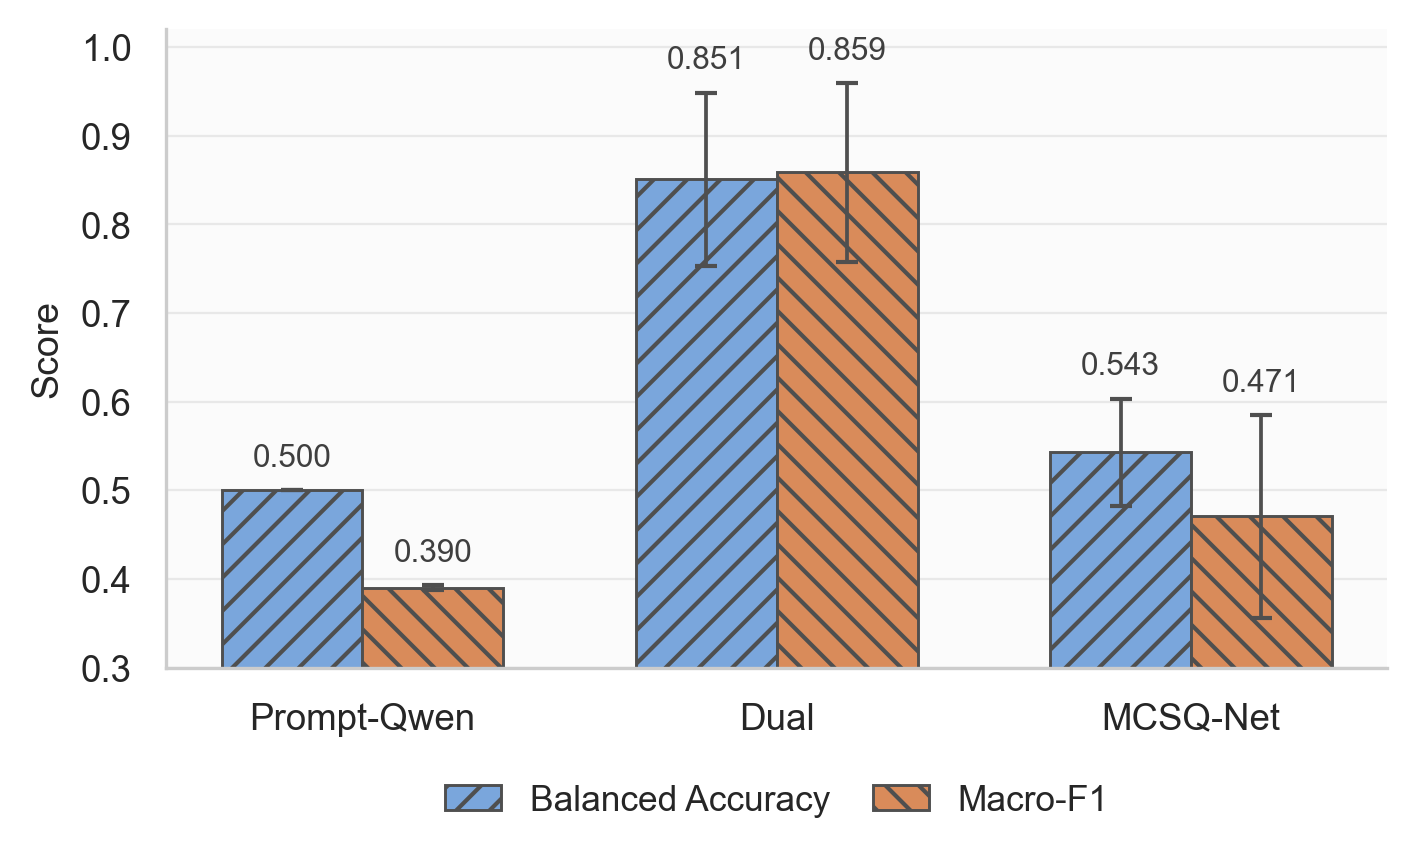
\includegraphics[width=0.9\columnwidth]{fig6.png}
\caption{Task-2 source-domain unseen-condition anomaly recognition results. Prompt-Qwen, the best classical baseline \texttt{Dual}, and MCSQ-Net are compared on Balanced Accuracy and Macro-F1. Error bars denote standard deviation over three folds.}
\label{fig:task2_anomaly_cn}
\end{figure}

Task-3 provides a stricter test through external transfer. Here the model faces simultaneous shifts in imaging conditions, process-parameter ranges, and defect distribution, so any reliance on condition-dependent surface cues is more likely to be exposed. Fig.~\ref{fig:data2_transfer_cn} shows the performance trajectories of three representative methods from Task-1 to Task-3. Prompt-Qwen remains weak in both domains. The strongest classical transfer baseline, \texttt{Tri-LF}, drops from 0.7751 to 0.4236 in Macro-F1 and from 0.7786 to 0.4973 in Balanced Accuracy. MCSQ-Net, by contrast, still attains a Macro-F1 of 0.6067 and a Balanced Accuracy of 0.6359, with a markedly smaller cross-domain degradation. This pattern is consistent with the intended role of the causal consistency constraint: it reduces the impact of condition-related spurious cues on the fused representation.

\begin{figure}[!t]
\centering
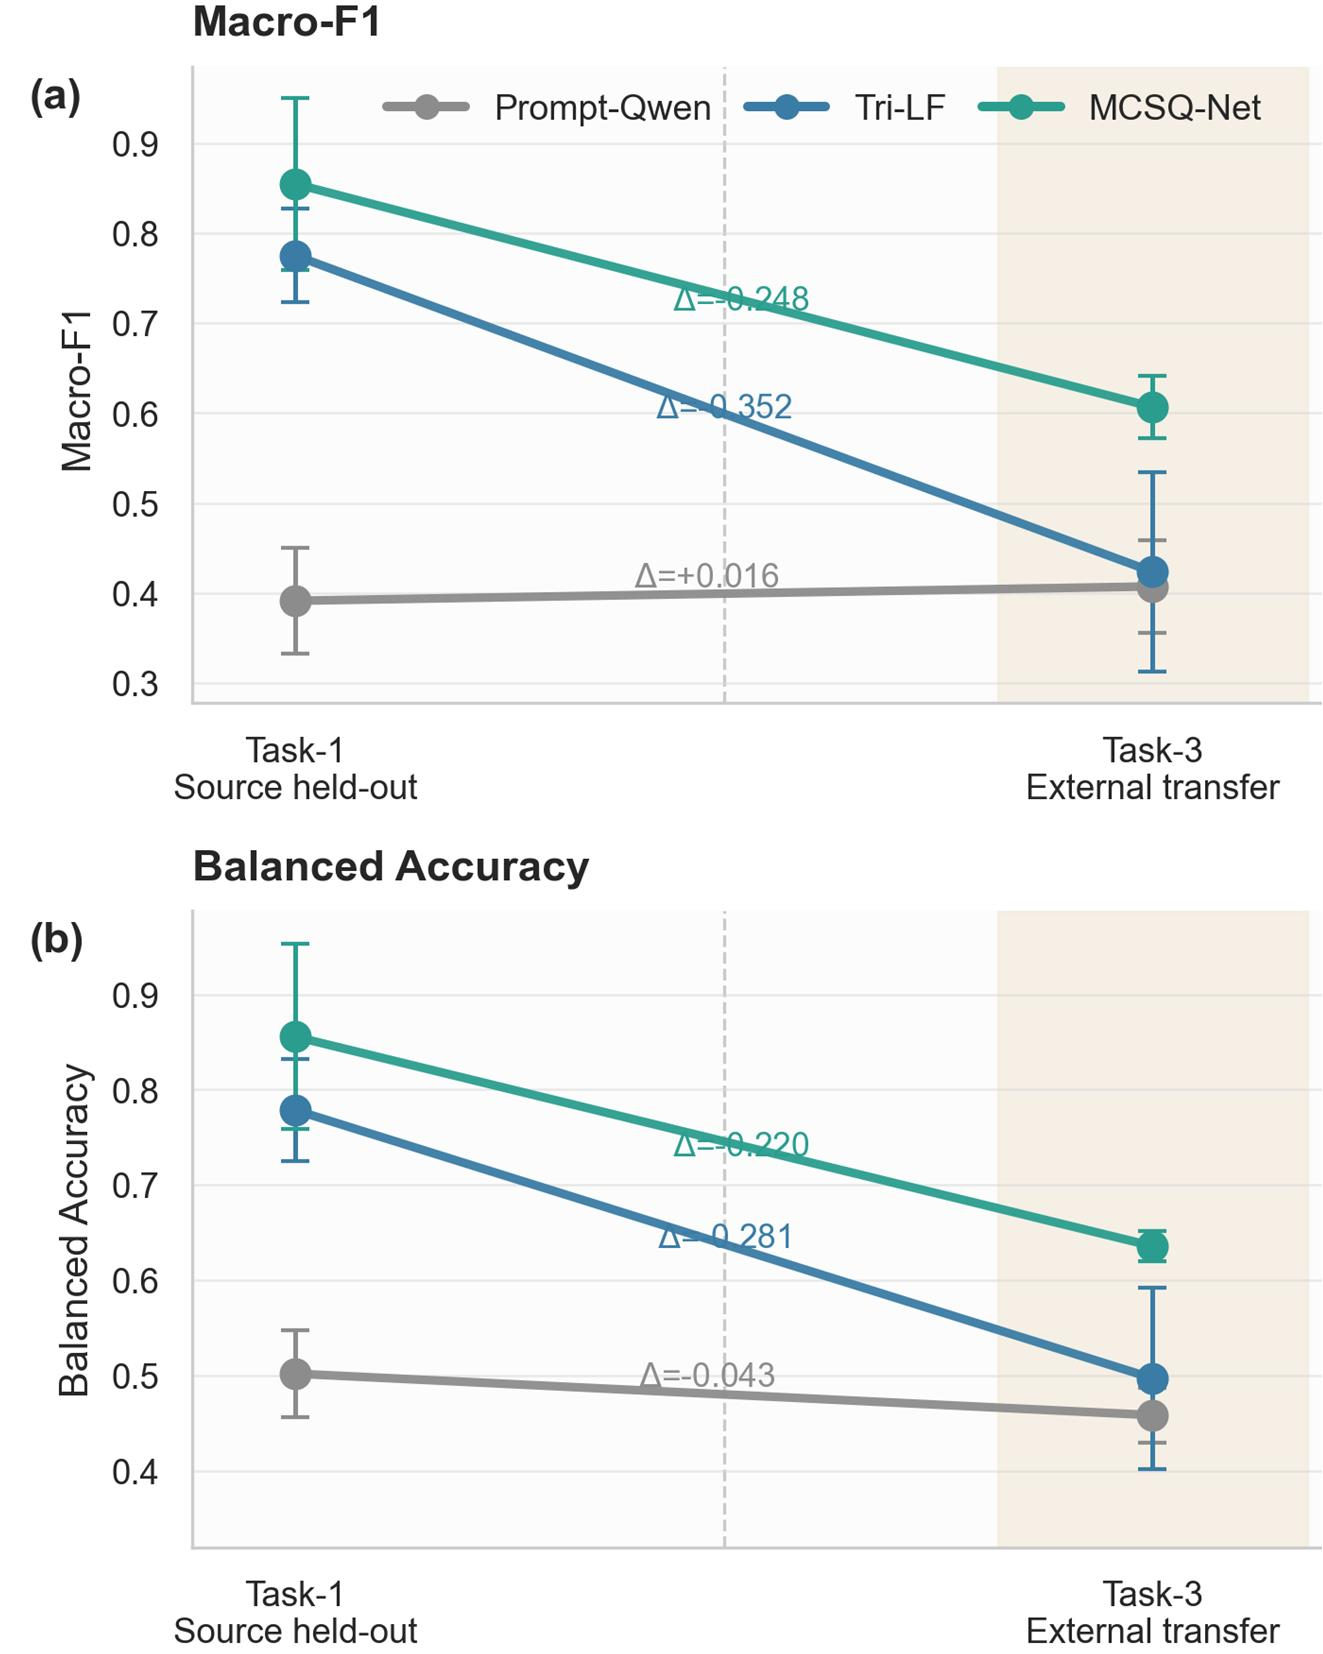
\includegraphics[width=0.9\columnwidth]{fig5.jpg}
\caption{Task-3 external-transfer defect category recognition results and cross-domain degradation. Top: Macro-F1. Bottom: Balanced Accuracy. Each trajectory connects the Task-1 source-domain result to the Task-3 external-transfer result. Error bars denote standard deviation over three folds, and the shaded region indicates the external target domain.}
\label{fig:data2_transfer_cn}
\end{figure}

This result also clarifies how the infrared modality contributes. Infrared information retains clear physical and statistical meaning in additive manufacturing monitoring \cite{ref_lpbf_sensing_review,ref_intelligent_defect_pbf}, but its benefit depends on the fusion mechanism and sample regime. In the classical transfer family, \texttt{Tri-LF} benefits from late fusion across three modalities, indicating that the way thermal information is exploited remains closely tied to the model family.

\subsection{Ablation Studies}

To clarify where the gains of MCSQ-Net come from, we conduct ablations from two angles: modality configuration and model structure. The results are summarized in Table~\ref{tab:ablation_cn}. The input ablation shows that each modality carries useful defect information, although its value depends on how fusion is performed. Infrared alone still reaches a Macro-F1 of 0.6270, which confirms that thermal information has standalone discriminative value. Among the tested input settings, the dual-camera configuration is the most stable, suggesting that complementary geometry and texture cues from two viewpoints are particularly well matched to the current task. Adding infrared through direct fusion does not improve the result further, implying that the present limitation lies less in whether infrared is included than in how its contribution is modeled. This reading is consistent with the transfer baselines, where the strongest classical method uses late fusion over three modalities. The model ablation points to the same conclusion. Removing the causal consistency constraint lowers Macro-F1 and Balanced Accuracy from 0.8547 and 0.8556 to 0.8402 and 0.8422, respectively. Unfreezing the last two visual blocks further reduces Macro-F1 to 0.7781, and also lowers Task-3 Macro-F1 from 0.6067 to 0.5808. The more effective strategy, therefore, is not aggressive backbone fine-tuning, but improving fusion-space stability while keeping the large-model prior intact.

\begin{table}[!t]
\caption{Ablation Results of MCSQ-Net}
\label{tab:ablation_cn}
\centering
\footnotesize
\setlength{\tabcolsep}{3pt}
\begin{tabular*}{\columnwidth}{@{\extracolsep{\fill}}>{\raggedright\arraybackslash}p{0.16\columnwidth}>{\raggedright\arraybackslash}p{0.34\columnwidth}>{\centering\arraybackslash}p{0.21\columnwidth}>{\centering\arraybackslash}p{0.21\columnwidth}@{}}
\toprule
Ablation Type & Setting & Balanced Accuracy & Macro-F1 \\
\midrule
\multirow{5}{=}{Input ablation}
& Camera 1 & 0.7714 $\pm$ 0.0771 & 0.7419 $\pm$ 0.1203 \\
& IR & 0.6508 $\pm$ 0.0708 & 0.6270 $\pm$ 0.0878 \\
& Camera 1 \& 2 & 0.8422 $\pm$ 0.1061 & 0.8402 $\pm$ 0.1048 \\
& Camera 1 \& 2 + IR & 0.8169 $\pm$ 0.0659 & 0.8121 $\pm$ 0.0615 \\
& Camera 1 \& 2 + causal consistency & \textbf{0.8556 $\pm$ 0.0973} & \textbf{0.8547 $\pm$ 0.0955} \\
\midrule
\multirow{3}{=}{Model ablation}
& w/o causal consistency & 0.8422 $\pm$ 0.1061 & 0.8402 $\pm$ 0.1048 \\
& Full model & \textbf{0.8556 $\pm$ 0.0973} & \textbf{0.8547 $\pm$ 0.0955} \\
& Unfreeze the last two visual blocks & 0.7979 $\pm$ 0.0332 & 0.7781 $\pm$ 0.0411 \\
\bottomrule
\end{tabular*}
\end{table}

\section{Conclusion}

This paper studied multimodal defect recognition in metal additive manufacturing under unseen conditions, with a particular focus on how pretrained large-model priors can improve cross-condition stability. To this end, MCSQ-Net was proposed to learn stable defect representations through shared visual encoding, multimodal fusion, and a cross-condition causal consistency constraint. Experimental results show that the method outperforms Prompt-Qwen and classical multimodal baselines in both source-domain unseen-condition defect category recognition and external transfer evaluation. This indicates that prompting alone or conventional multimodal fusion is insufficient to cope with condition shift, whereas explicitly suppressing condition-related spurious cues in the fused representation is critical for generalization. Ablation studies further show that the causal consistency constraint consistently improves representation quality, while aggressively unfreezing the visual backbone weakens the original pretrained prior and leads to overfitting. Future work will investigate finer-grained fusion mechanisms for infrared thermal features and more conservative parameter-efficient adaptation strategies on the visual side, such as adapters or LoRA modules.

\begin{thebibliography}{00}

\bibitem{ref_defect_formation_slm}
B.~Zhang, Y.~Li, and Q.~Bai, ``Defect formation mechanisms in selective laser melting: A review,'' \emph{Chinese Journal of Mechanical Engineering}, vol.~30, pp.~515--527, 2017.

\bibitem{ref_in_situ_monitoring_review}
X.~Peng, L.~Kong, H.~An, and G.~Dong, ``A review of in situ defect detection and monitoring technologies in selective laser melting,'' \emph{3D Printing and Additive Manufacturing}, vol.~10, no.~3, pp.~438--466, 2023.

\bibitem{ref_lpbf_sensing_review}
D.~Guillen, S.~Wahlquist, and A.~Ali, ``Critical review of LPBF metal print defects detection: Roles of selective sensing technology,'' \emph{Applied Sciences}, vol.~14, no.~15, p.~6718, 2024.

\bibitem{ref_intelligent_defect_pbf}
P.~Wang \emph{et al.}, ``Towards intelligent defect detection in metal powder bed fusion: A review of in situ monitoring, data pre-processing, and machine learning,'' \emph{Materials Science and Engineering: R: Reports}, vol.~167, p.~101112, 2026.

\bibitem{ref_anomalygpt}
Z.~Gu \emph{et al.}, ``AnomalyGPT: Detecting industrial anomalies using large vision-language models,'' arXiv:2308.15366, 2023.

\bibitem{ref_myriad}
Y.~Li \emph{et al.}, ``Myriad: Large multimodal model by applying vision experts for industrial anomaly detection,'' arXiv:2310.19070, 2023.

\bibitem{ref_vlm_active_learning}
S.~Chen and Y.~Liu, ``Vision-language model-assisted active learning for high-accuracy defect detection in automotive bushing components,'' in \emph{Proc. Int. Conf. Embodied Intelligence and Large Models}, 2025, pp.~9--14.

\bibitem{ref_qlora_excavator}
H.~V.~Nguyen, H.~Park, N.~Yoo, and J.~Yang, ``Resource-efficient fine-tuning of large vision-language models for multimodal perception in autonomous excavators,'' \emph{Frontiers in Artificial Intelligence}, vol.~8, p.~1681277, 2025.

\bibitem{ref_omniad}
S.~Zhao \emph{et al.}, ``OmniAD: Detect and understand industrial anomaly via multimodal reasoning,'' arXiv:2505.22039, 2025.

\bibitem{ref_ad_copilot}
X.~Jiang \emph{et al.}, ``AD-Copilot: A vision-language assistant for industrial anomaly detection via visual in-context comparison,'' arXiv:2603.13779, 2026.

\bibitem{ref_wu2024_multisensor}
Q.~Wu \emph{et al.}, ``In-situ quality intelligent classification of additively manufactured parts using a multi-sensor fusion based melt pool monitoring system,'' \emph{Additive Manufacturing Frontiers}, vol.~3, no.~3, p.~200153, 2024.

\bibitem{ref_liu2024_acoustic}
H.~Liu \emph{et al.}, ``Inference of highly time-resolved melt pool visual characteristics and spatially-dependent lack-of-fusion defects in laser powder bed fusion using acoustic and thermal emission data,'' \emph{Additive Manufacturing}, vol.~83, p.~104057, 2024.

\bibitem{ref_shen2024_multisource}
T.~Shen \emph{et al.}, ``Multi-source information fusion for enhanced in-process quality monitoring of laser powder bed fusion additive manufacturing,'' \emph{Additive Manufacturing}, vol.~96, p.~104575, 2024.

\bibitem{ref_li2024_transfer}
J.~Li \emph{et al.}, ``Transfer learning-based quality monitoring of laser powder bed fusion across materials,'' \emph{Expert Systems with Applications}, vol.~252, p.~124150, 2024.

\end{thebibliography}

\end{document}
